\documentclass{article}

%%%%%%%%%%%%%%%%%%%%%%%%%%%%%%%%%%%%%%%%%%%%%%%%%%%%%
%                                                   %
%              Template by Tuur Vanhoutte           %
% https://github.com/zjeffer/howest-thesis-template %
%                                                   % 
%%%%%%%%%%%%%%%%%%%%%%%%%%%%%%%%%%%%%%%%%%%%%%%%%%%%%

%%%%% Package importing %%%%%
\usepackage[english]{babel}
\usepackage[margin=2.5cm]{geometry}
\usepackage{graphicx}
\usepackage{float}
\usepackage{caption}
\usepackage{hyperref}
\usepackage{amsmath}
\usepackage{wrapfig}
\usepackage[parfill]{parskip}
\usepackage{eso-pic}
\usepackage{titlesec}
\usepackage{titletoc}
\usepackage{tcolorbox}
\usepackage{enumitem}
\usepackage{changepage}

\usepackage{bookmark}
\usepackage{csquotes}
\usepackage[style=ieee]{biblatex}
\addbibresource{sources.bib}



%%%%% Change fonts here %%%%%
\usepackage[T1]{fontenc}
\usepackage{helvet}
\renewcommand{\familydefault}{\sfdefault}

\graphicspath{{img/}}

%%%%% \theorem environment %%%%%
\usepackage{amssymb}
\newtheorem{theorem}{Definition}[section]
\newenvironment{thmenum}
 {\begin{enumerate}[label=\upshape\bfseries(\roman*)]}
 {\end{enumerate}}


%%%%% Styled code block %%%%%
\usepackage{minted}
\setminted{frame=single,framesep=3pt,linenos}
\usepackage{upquote}
\usepackage{color}

%%%%% TOC styling %%%%%
\makeatletter
\renewcommand\tableofcontents{%
  \null\hfill\textbf{\Huge\contentsname}\hfill\null\par
  \vline\noexpand\rule{\textwidth}{1pt}%
  \@mkboth{\MakeUppercase\contentsname}{\MakeUppercase\contentsname}%
  \@starttoc{toc}%
}
\makeatother



\begin{document}

%%%%% title page %%%%%
\begin{titlepage}
    \newgeometry{margin=0cm}
    \begin{center}
        %%%%% Change the cover image here %%%%%
        \includegraphics[width=18.5cm,height=18.5cm]{example-image}
    \end{center}
    \begin{adjustwidth}{1.5cm}{1.5cm}

    \vspace{0.5em}

    \MakeUppercase{\Huge\textbf{How to create a chess engine using Deep Reinforcement Learning}}

    \MakeUppercase{\Large\textit{A critical look at DeepMind's AlphaZero}}

    \vspace{1em}

    \MakeUppercase{Interal promotor: Wouter Gevaert}

    \MakeUppercase{External promotor: <name here>}

    \vspace{1em}

    \MakeUppercase{\small{Research conducted by}}

    \MakeUppercase{\Large\textbf{{Tuur Vanhoutte}}}

    \MakeUppercase{\small{for obtaining a bachelor's degree in}}

    \MakeUppercase{\Large{\textbf{{Multimedia \& Creative Technologies}}}}

    \MakeUppercase{Howest | 2021-2022}
    \end{adjustwidth}
\end{titlepage}

\newgeometry{margin=2.5cm}

\newpage
\thispagestyle{empty}
\mbox{}
\newpage

%%%%% Set pagenumbering off %%%%%
\pagenumbering{arabic}
\thispagestyle{empty}
%%%%% Preface %%%%%
\section*{Preface}
\addcontentsline{toc}{section}{Preface}

This bachelor thesis is the conclusion to the bachelor programme Multimedia \& Creative Technologies at Howest college
West Flanders in Kortrijk, Belgium. The programme teaches students a wide range of skills in the field of 
computer science, with a focus on creativity and Internet of Things. From the second year on, students can choose 
between four different modules:

\begin{enumerate}
    \item \textbf{AI Engineer}
    \item \textbf{Smart XR Developer}
    \item \textbf{Next Web Developer}
    \item \textbf{IoT Infrastructure Engineer}
\end{enumerate}

This bachelor thesis was made under the \textbf{AI Engineer} module.
The subject of the thesis is a critical look at the result of my research project 
in the previous semester. The goal of the project was to create a chess engine in Python with
deep reinforcement learning based on DeepMind's AlphaZero algorithm. 

I will explain the research I needed to create it, the technical details on how to program the
chess engine and I will reflect on the results of the project. To do this, I will contact 
multiple people familiar with the field of reinforcement learning to get a better understanding of the
impact of this research on society. Based on this, I will give advice to people and companies who 
wish to implement similar algorithms.

I would like to show gratitude to Wouter Gevaert for his enthousiastic support in the creation of my research project 
and this thesis. I also want to thank the other teachers at Howest Kortrijk, who shared their knowledge
and expertise in programming and AI in very interesting classes.

% TODO: thank external promotor

Furthermore, I would liike to thank my parents for giving me the chance to have a good education, and 
the motivation to get the best I can out of my studies.

\vspace{3em}

\begin{center}
    \textbf{Tuur Vanhoutte}, 1$^{\text{st}}$ June 2022 % TODO: verander datum naar datum finale versie
\end{center}

\newpage
\thispagestyle{empty}
\mbox{}
\newpage

%%%%% Abstract %%%%%
\section*{Abstract}
\addcontentsline{toc}{section}{Abstract}


% TODO: abstract verder aanvullen

% Samenvatting of abstract (mag in het Engels): MAX 1 halve A4-pagina: 
% Je beantwoordt in de samenvatting kort en bondig een viertal vragen: 
% X Wat is de onderzoeksvraag?
% X Wat was jouw onderzoek? 
% - Welke elementen spelen een grote rol (zowel positief als negatief) bij de evaluatie van het onderzoek? 
% - Welke elementen zijn belangrijk bij jouw advies?
% - Het besluit wordt kort samengevat

This bachelor thesis answers the question: ``How to create a chess engine using deep reinforcement learning?''.
It explains the difference between normal chess engines and chess engines that use deep reinforcement learning, and
specifically tries to recreate the results of AlphaZero, the chess engine by DeepMind, in Python on consumer hardware. 

The technical research shows what is needed to create my implementation using Python and TensorFlow. 
It shows how to program the chess engine, how to build the neural network, and how to train and evaluate the network.
During the creation of this chess engine, it was crucial to create a huge amount of data through self-play.

The thesis contains a reflection on the results of my research project, which proposes a solution to the problem of
creating a high amount of games through self-play. It also reflects on the impact of this research on society, and the
viability of this type of artificial intelligence in the future. With this comes a section on advice for companies that wish
to implement similar algorithms.

% It concludes... (TODO)


\newpage
\thispagestyle{empty}
\mbox{}
\newpage

%%%%% Table of contents %%%%%
\addcontentsline{toc}{section}{Contents}
\tableofcontents
\newpage

%%%%% List of figures %%%%%
\section*{List of figures}
\addcontentsline{toc}{section}{List of figures}
\renewcommand{\listfigurename}{}
\listoffigures

% TODO: Remove if no tables
% \section*{List of tables}
% \addcontentsline{toc}{section}{List of tables}
% \renewcommand{\listtablename}{}
% \listoftables

%%%%% List of abbreviations %%%%%
\section*{List of abbreviations}
\addcontentsline{toc}{section}{List of abbreviations}

%%%%% Glossary %%%%%
\newpage
\section*{Glossary}
\addcontentsline{toc}{section}{Glossary}

%%%%% Introduction %%%%%
\newpage
\setcounter{section}{0}
\section{Introduction}

% Doel: In de inleiding beschrijf je ook hoe jouw bachelorproef in elkaar steekt. Een krachtige heldere inleiding 
% zorgt ervoor dat je de lezer voor je wint en hij/zij sneller de rest van jouw document zal gaan lezen. 
% In de inleiding introduceer je de onderzoeksvraag. Je vermeldt de achtergrond of bestaande situatie. Je licht toe 
% waarom de onderzoeksvraag voor jou/jouw stagebedrijf relevant is. Ook eventuele deelvragen worden 
% nauwgezet omschreven. 
% De inleiding omschrijft ook de gebruikte onderzoeksmethode. Je legt uit waar, wanneer, met wie en hoe je het 
% onderzoek gaat doen. 
% Je kunt alvast gebruikmaken van één of meerdere standaardzinnen: 
% - De data voor dit onderzoek zijn verzameld door... 
% - Vijf stukken worden onderzocht, die allemaal... 
% - De onderzoeksgegevens in deze bachelorproef zijn afkomstig uit vier belangrijke bronnen, namelijk... 
% - Door kwalitatieve methoden te gebruiken probeer ik... uiteen te zetten/uit te lichten. 
% - De studie is uitgevoerd in de vorm van een enquête, waarbij data zijn verzameld via... 
% - De methode die in deze studie gebruikt is, is een gemengde aanpak gebaseerd op...

Chess is not only one of the most popular board games in the world, it is also a breeding ground for
complex algorithms and more recently, machine learning. Chess is theoretically a deterministic game: 
no information is hidden from either player and every position has a calculable set of possible moves.
Because the branching factor of chess is about 35-38 moves \cite{BranchingFactorChessprogramming}, 
calculating if a position is winning or losing requires an enormous amount of calculations.

Throughout the entire history of computer science, researchers have continously tried to find better
ways to calculate if a position is winning or losing. The most famous example is the StockFish 
engine \cite{StockfishChess2022}, which uses the minimax algorithm with alpha-beta pruning to calculate the best move.

More recently, researchers at Google DeepMind have developed a new algorithm called AlphaZero \cite{AlphaZero2022}.
This thesis explores the concept of AlphaZero, how to create a chess engine based on it, and the impact of 
the algorithm on both the world of chess and the rest of society.

Research has been conducted by investigating what is needed to recreate the results of AlphaZero, 
by programming a simple implementation using Python and TensorFlow. This was done as part of a research project
between November 2021 and January 2022. The code was written with lots of trial and error, as DeepMind released 
very little information about the detailed workings of the algorithm. 

% TODO: more info


%%%%% Add Howest background %%%%%
\AddToShipoutPicture{
    \ifnum\value{page}>0
    \AtPageLowerLeft{
    \raisebox{3\baselineskip}{\makebox[0.25\paperwidth]{
        \begin{minipage}{21cm}\centering
            
\includegraphics{img/background.png}
        \end{minipage}}}
    }
  \fi
}

%%%%% Research %%%%%
\newpage
\section{Research}

%%%%%%%%%%%%% 
% 
% Answer the theoretical questions:
%
% [ ] Hoe kan ik het Monte Carlo Tree Search algoritme gebruiken om de beste zetten te selecteren?
% [ ] Welke voordelen biedt deep reinforcement learning bij schaken?
% [ ] Hoe ziet de architectuur van het neurale netwerk er uit?
% [ ] Hoe werd deep reinforcement learning reeds gebruikt bij andere spellen?
% [ ] Hoe werken huidige schaakcomputers die geen neurale netwerken gebruiken?
% [ ] Hoe kan ik met normale hardware een deep reinforcement learning schaakcomputer trainen? Wat zijn de limitaties?
% [ ] Kan ik mijn schaakcomputer beter maken dan een amateurspeler (1000 ELO)?
%
%%%%%%%%%%%%%

\subsection{What is a chess engine?}

According to Wikipedia \cite{ChessEngine2022}, a chess engine is a computer program that analyzes 
chess or chess variant positions, and generates a move or list of moves that it regards as strongest.
Given any chess position, the engine will estimate the winner of that position based on the strength 
of the possible future moves up to a certain depth. The strength of a chess engine is determined by
the amount of moves, both in depth and breadth, that the engine can calcuate. 


\subsection{How do traditional chess engines work?}

Contemporary chess engines, like Stockfish, use a variant of the minimax algorithm that employs alpha-beta pruning.

\subsubsection{The minimax algorithm}

The minimax algorithm \cite{Minimax2022} is a general algorithm usable in many applications, ranging from artificial intelligence to 
decision theory and game theory. The algorithm tries to minimize the maximum amount of loss. In chess, this means 
that the engine tries to minimize the possibility for the worst-case scenario: the opponent
checkmating the player. For games where the player needs to maximize a score, the algorithm is called maximin: 
maximizing the minimum gain. 

Minimax creates a tree with chess positions as nodes and chess moves as edges between the nodes. 
Each node gets a value that represents the strength of the position for the current player. 
It starts with only the root of the tree as the current position. 
The algorithm explores the tree in a depth-first manner. 
This means that it will traverse the tree vertically until a certain depth is reached. When that happens, the algorithm evaluates that node's
position and returns its value to its parent node. % TODO: more info

\begin{figure}[H]
    \centering
    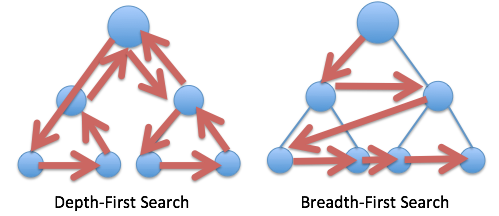
\includegraphics[width=0.5\textwidth]{img/depth-vs-breadth.png}
    \caption{Depth-First search vs Breadth-First search \cite{eppesHowComputerizedChess2019}}
\end{figure}












\subsubsection{Pseudocode}

The algorithm is recursive: it calls itself with different arguments, depending
on which player's turn it is. In chess, white wants to maximize the score, and 
black wants to minimize it. \cite{Minimax2022}

\begin{minted}{c}
function  minimax(node, depth, maximizingPlayer) is
    if depth = 0 or node is a terminal node then
        return the heuristic value of node
    if maximizingPlayer then
        value := - inf
        for each child of node do
            value := max(value, minimax(child, depth - 1, FALSE))
        return value
    else (* minimizing player *)
        value := + inf
        for each child of node do
            value := min(value, minimax(child, depth - 1, TRUE))
        return value
\end{minted}

Calling the function:

\begin{minted}{c}
minimax(origin, depth, TRUE)
\end{minted}



\subsubsection{Alpha-beta pruning}

Alpha-beta pruning is an algorithm \cite{AlphaBetaPruning2022} to reduce the amount of nodes that need to be evaluated by minimax.
It does this by cutting away tree branches that lead to worse outcomes. 




\subsection{AlphaZero}



%%%%% Technical research %%%%%
\newpage
\section{Technical research}

%%%%% Reflection %%%%%
\newpage
\section{Reflection}

%%%%% Advice %%%%%
\newpage
\section{Advice}

%%%%% Conclusion %%%%%
\newpage
\section{Conclusion}

%%%%% Bibliography %%%%%
\newpage
\section{Bibliography}
\renewcommand{\bibname}{}
\printbibliography[heading=none]

%%%%% Appendix %%%%%
\newpage
\section{Appendix}





\end{document}